\documentclass[11pt]{beamer}
\usetheme{CambridgeUS}
\usepackage[utf8]{inputenc}
\usepackage{amsmath}
\usepackage{amsfonts}
\usepackage{amssymb}
\usepackage{graphicx}
\author{Will Gertsch}
\title{D-optimal Designs for Logistic Models using Metaheuristics}
%\setbeamercovered{transparent} 
%\setbeamertemplate{navigation symbols}{} 
%\logo{} 
%\institute{} 
%\date{} 
%\subject{} 
\begin{document}

\begin{frame}
\titlepage
\end{frame}

%\begin{frame}
%\tableofcontents
%\end{frame}

\begin{frame}{Outline}
\begin{enumerate}
\item Logistic regression model and information matrix
\item Optimal design background
\item Particle swarm and genetic algorithm
\item D-optimal designs for a linear predictor
\item D-optimal designs for a quadratic predictor
\end{enumerate}
\end{frame}

\begin{frame}{Logistic Model}
Suppose $y_i \sim \text{Bernoulli}(p_i)$ for $i = 1, \dots, n$. The logit link function is defined as
$$
p_i = \frac{1}{1+e^{-\eta_i}} = \frac{e^{\eta_i}}{1+e^{\eta_i}}
$$
where $\eta_i = \beta_0  + \beta_1 x_{i}$
and $0 \leq p_i < 1$

We may also use a quadratic model $\eta_i = \beta_0  + \beta_1 x_{i} + \beta_2 x_i^2$.
\end{frame}

\begin{frame}{Information Matrix}
The information matrix for the logistic model can be derived as 
$$
M(\beta) = \sum_{i=1}^k p_i (1-p_i) f(x_i) f(x_i)' = X'WX
$$
where $W$ is a diagonal weight matrix with entries $p_i (1-p_i)$. The design matrix $X$ has rows $f(x_i)' = (1, x_i)$ if $\eta_i$ is linear. If $\eta_i$ is quadratic, then $f(x_i)' = (1,x_i,x_i^2)$. 
\end{frame}

%\begin{frame}{Information Matrix Example}
%Suppose we have $\eta_i = \beta_0 + \beta_1 x_i$ and $n = 2$. Then the information matrix is
%$$
%I\begin{pmatrix}
%\beta_0\\
%\beta_1
%\end{pmatrix}
%=
%p_1 (1-p_1)
%\begin{pmatrix}
%1 & x_1\\
%x_1 & x_1^2
%\end{pmatrix}
%+
%p_2 (1-p_2)
%\begin{pmatrix}
%1 & x_1\\
%x_1 & x_1^2
%\end{pmatrix}
%$$
%Note that  $I$ depends on $\beta_0$ and $\beta_1$ through $p_1$ and $p_2$.
%
%\end{frame}

\begin{frame}{Design Notation}
We denote a design $\xi$ using weight notation. If we have $N$ samples total and $n_i$ samples for each design point $x_1 \dots, x_k$, let 
$$
\xi =
\begin{pmatrix}
x_1 & \dots & x_k\\
w_1 & \dots & w_k
\end{pmatrix}
$$
where $w_i = n_i/N$ are weights.
\end{frame}


\begin{frame}{Information Matrices}
In optimal design, a design $\xi$  implies a corresponding information matrix
$$
M = M(\xi, \beta) = \sum_{i=1}^k w_ip_i (1-p_i) f(x_i) f(x_i)' = X'WX
$$
where $W$ now has diagonal entries $w_i p_i (1-p_i)$
\end{frame}

\begin{frame}{Locally Optimal Designs}
For a given value of the parameter vector $\beta$, we can find a locally optimal design by minimizing functions of the information matrix. Below are some common examples:
\begin{itemize}
\item \textbf{D-optimality:} $-\log\left(\text{det}(M)\right)$
\item A-optimality: $\text{tr}(M^{-1})$
\item E-optimality: $-\text{max}_{M} \text{min}_{Mv = \lambda v} \lambda$
\end{itemize}


In this presentation, we will focus on D-optimality.
\end{frame}

\begin{frame}{Equivalence Theorem for D-optimality}
We can test if a design is D-optimal by computing the sensitivity function
$$
ch(x) = g(x) f(x)'M(\xi, \beta)^{-1} f(x) - p
$$
where $p$ is the number of parameters in the model and 
$$
g(x) = \frac{\exp(\eta)}{(1+\exp(\eta))^2}
$$
$\eta = \beta_0  + \beta_1 x$ or $\eta = \beta_0 + \beta_1 x + \beta_2 x^2$
\end{frame}

\begin{frame}{Plotting ch(x)}
If $ch(x) = g(x) f(x)'M(\xi, \beta)^{-1} f(x) - p \leq 0$ with equality at the design points, then the design $\xi$ is D-optimal. In other words, we can plot $ch(x)$ to see if a design is optimal.\\


\begin{figure}[h]
\centering
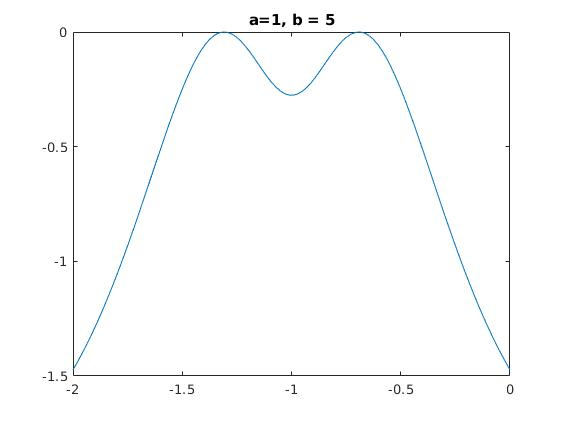
\includegraphics[scale=0.3]{prob3p2.jpg}
\caption{ch(x) for a D-optimal design}

\end{figure}

\end{frame}

\begin{frame}{Review of Previous Results}
Papers on the logistic model D-optimality:
\begin{itemize}
\item Mathew, Sinha (2001) derive D-optimal designs for linear $\eta$.
\item Sebastiani, Settimi (1992) derive designs on different design intervals for linear $\eta$.
\item Lall et al. (2018) use a Fedorov algorithm to find designs on $[-1,1]$.
\item Fornius (2005) found designs numerically for quadratic $\eta$.
\end{itemize}
\end{frame}

\begin{frame}{My Contributions}
I wrote software that uses metaheuristic optimization algorithms to
\begin{itemize}
\item Find D-optimal designs for linear and quadratic logistic models.
\item Find designs on any design interval.
\item Change number of design points.
\end{itemize}
\end{frame}

\begin{frame}{Choice of algorithm}
I used 2 algorithms to find designs:
\begin{itemize}
\item Particle swarm optimization (PSO)
\item Genetic algorithm (GA)
\item Using implementation in PlatEMO with default parameters.
\item PSO may work better than GA or vice-versa
\end{itemize}
These algorithms were chosen because they worked the best out of all the other single-objective algorithms in PlatEMO for this problem.
\end{frame}

\begin{frame}{Particle Swarm Optimization}
Particle swarm optimization (PSO) (Kennedy, Ebernhart 1995) is a nature-inspired algorithm to find the optimal value of an objective function. It is based on fish and bird schooling behavior.\\
\textbf{Algorithm}:
\begin{enumerate}
\item Initialize $N$ particles $x_i$ with velocities $v_i$.
\item Find particle with best objective value.
\item Update velocity $v_i^{t+1}$ for all particles such that they are drawn towards the current best global value and towards the current best for particle $i$.
\item Update location $x_i^{t+1} = x_i^{t} + v_i^{t+1}$ for all particles.
\item Repeat steps 2-4.
\end{enumerate}
%PlatEMO: Velocity calculation includes a constant inertial weight that can be specified by user.
\end{frame}

\begin{frame}{Genetic Algorithm}
The genetic algorithm (GA) (Holland 1975) is based on natural selection.It has 3 main steps: crossover, mutation, and selection.
\begin{itemize}
\item $x_i$'s are encoded as strings called chromosomes.
\item Crossover and mutation steps operate on these chromosomes.
\item Diagrams from \textit{Nature-Inspired Optimization Algorithms} by Xin-She Yang.
\end{itemize}
\end{frame}

\begin{frame}{Crossover}

\centering
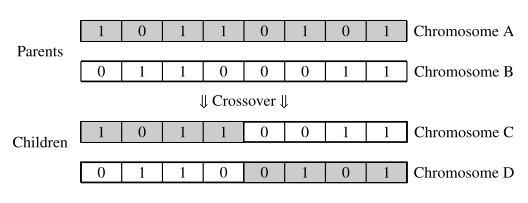
\includegraphics[scale=0.5]{crossover.png}


\end{frame}

\begin{frame}{Mutation}
\centering
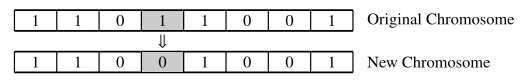
\includegraphics[scale=0.5]{mutation.png}
\end{frame}

\begin{frame}{Genetic Algorithm}
\textbf{Algorithm}:
\begin{enumerate}
\item Initialize $N$ solutions.
\item Crossover: swap characteristics of 2 parent solutions with prob. $p_c$ to produce 2 child solutions.
\item Mutation: randomly alter a characteristic of a child solutions with prob. $p_m$.
\item Selection: Accept child solutions if fitness increases.
\item Best $N$ solutions go on to next generation.
\item Repeat steps 2-5.
\end{enumerate}
This is the basic format of a genetic algorithm. Details may vary with implementation.
\end{frame}

\begin{frame}{Results from Mathew, Sinha}
Mathew, Sinha show that the locally $D$-optimal design for a logistic model with $\eta = \beta_0 + \beta_1 x$ has two equally weighted design points
$$
x_1, x_2 = \frac{\pm 1.5434 - \beta_0}{\beta_1}
$$
\end{frame}

\begin{frame}{Results from Mathew, Sinha}
Algorithms were run with swarm size of 1000 and for 1000000 objective function evaluations. Both algorithms had the same initial values.
\begin{tabular}{|c|c|c|c|}
\hline 
$\beta$ & Theoretical & PSO & GA \\ 
\hline 
0,1 & $\begin{bmatrix}
-1.5434 & 1.5434\\ 0.5 & 0.5
\end{bmatrix}$ & $\begin{bmatrix}
-1.5434 & 1.5434\\ 0.5000 & 0.5000
\end{bmatrix}$ & $\begin{bmatrix}
-1.5452 & 1.5435\\ 0.5000 & 0.5000
\end{bmatrix}$ \\ 
\hline 
0.3,0.4 & $\begin{bmatrix}
-4.6085 & 3.1085\\ 0.5 & 0.5
\end{bmatrix}$ & $\begin{bmatrix}
-4.6085 & 3.1085\\ 0.5000 & 0.5000
\end{bmatrix}$ & $\begin{bmatrix}
-4.6091 & 3.1083\\ 0.5000 & 0.5000
\end{bmatrix}$ \\ 
\hline 
2,-5 & $\begin{bmatrix}
0.0913 & 0.7087\\ 0.5 & 0.5
\end{bmatrix}$ & $\begin{bmatrix}
0.0913 & 0.7087\\ 0.5000 & 0.5000
\end{bmatrix}$ & $\begin{bmatrix}
0.0923 & 0.7109\\ 0.5000 & 0.5000
\end{bmatrix}$  \\ 
\hline 
\end{tabular} 

PSO tends to converge quicker for this problem but GA comes very close to theoretical solution.
\end{frame}

\begin{frame}{Results from Lall et al.}
Lall et. al use a modified Fedorov algorithm to find D-optimal designs on $[-1,1]$. PSO and GA are run with the same parameters as last slide.
\begin{tabular}{|c|c|c|c|c|c|c|c|}
\hline 
 $\beta_0$ & $\beta_1$ & $x_1 (F)$ & $x_2 (F)$ & $x_1 (PSO)$ & $x_2 (PSO)$ & $x_1 (GA)$ & $x_2 (GA)$\\
\hline 
 0.1 & 0.5 & -1 & 1 & -1 & 1 & -1 & 1\\ 
\hline 
 1 & 1 & -1 & 1 & -1 & 1 & -1 & 1\\ 
\hline 
 1 & 4 & -0.636 & 0.136 & -0.636 & 0.136 & -0.636 & 0.136\\ 
\hline 
\end{tabular}
PSO and GA both are able to confirm the solution.
\end{frame}

\begin{frame}{Results Sebastiani}
Sebastiani derives theoretical results for all possible combinations of design intervals. The resulting designs are modifications of the optimal design on $(-\infty, \infty)$. To illustrate, I selected $\beta_0 = 0, \beta_1=1$. All resulting designs were equally weighted.

\begin{tabular}{|c|c|c|c|c|c|}
\hline 
  & $[-\infty, \infty]$  & $[-1, \infty]$ & $[-\infty,1]$ & $[-1,1]$ & $[10, 20]$\\ 
\hline 
$x_1 (T)$ & -1.543 & -1 & -1.796 & -1  & ?\\ 
\hline 
$x_2 (T)$ & 1.543 & 1.796 & 1 & 1 & ?\\ 
\hline 
$x_1 (PSO)$ & -1.543 & -1 & -1.796 & -1 & $10^*$\\
\hline
$x_2 (PSO)$ & 1.543  & 1.796 & 1 & 1 & $10^*$\\
\hline
$x_1 (GA)$ & -1.545 & -1 & -1.796 & -1 & $10$\\
\hline
$x_2 (GA)$ & 1.544 & 1.796 & 1 & 1 & $12$\\
\hline
\end{tabular} \\
$*$ PSO had trouble converging to the correct solution in this case. \\Note also that the last case is not covered in Sebastiani.
\end{frame}

\begin{frame}{Results from Fornius}
Fornious (2005) derives D-optimal designs for the quadratic model with $\eta_i = \beta_0 + \beta_1 x_i + \beta_2 x_i^2$. Designs have either 3 or 4 support points depending on shape of response.

\begin{tabular}{|c|c|}
\hline 
 Nominal values & Design \\ 
\hline 
 $2,0,-0.1$ & 
$\begin{bmatrix}
-5.7185 & -2.7017  & 2.7017 & 5.7185\\
0.3138 & 0.1862 & 0.1862 & 0.3138
\end{bmatrix}$  \\ 
\hline 
 $2,0,-4$ & $\begin{bmatrix}
-0.9042 & -0.4272  & 0.4272 & 0.9042\\
0.3138 & 0.1862 & 0.1862 & 0.3138
\end{bmatrix}$   \\ 
\hline 
 $-2,0,-0.1$ & 
$\begin{bmatrix}
-3.9819 & 0  & 3.9819\\
1/3 & 1/3 & 1/3
\end{bmatrix}$   \\ 
\hline 
 $-2,0,-4$ & 
$\begin{bmatrix}
-0.6296 & 0  & 0.6296\\
1/3 & 1/3 & 1/3
\end{bmatrix}$  \\ 
\hline 
\end{tabular} \\
$\beta_1 \neq 0$ shifts the design.\\ What about on different design intervals?
\end{frame}

% better to just use plots for these designs
%\begin{frame}{Fornius PSO}
%PSO struggles to find the optimal design for the 4 point designs even after many iterations. 3 point designs seem to be easier.
%
%\begin{tabular}{|c|c|}
%\hline 
% Nominal values & Design \\ 
%\hline 
% $2,0,-0.1$ & 
%$\begin{bmatrix}
%-5.8244 & -1.6960  & 3.0160 & 5.5276\\
%0.3629 & 0.3006  & 0.0698 & 0.2668
%\end{bmatrix}$  \\ 
%\hline 
% $2,0,-4$ & $\begin{bmatrix}
%-0.9208 & -0.3372 & 0.7906 & 0.8980\\
%0.3355 & 0.3124 & 0.1645 & 0.1876 
%\end{bmatrix}$   \\ 
%\hline 
% $-2,0,-0.1$ & 
%$\begin{bmatrix}
%-3.9819 & 0  & 3.9819\\
%1/3 & 1/3 & 1/3
%\end{bmatrix}$   \\ 
%\hline 
% $-2,0,-4$ & 
%$\begin{bmatrix}
%-0.6295 & 0.0001  & 0.6297\\
%0.3346 & 0.3331 & 0.3323
%\end{bmatrix}$  \\ 
%\hline 
%\end{tabular} 
%\end{frame}
\begin{frame}{PSO Results 1}
PSO can find optimal designs for the 3 point cases.
\includegraphics[scale=0.28]{quadplots/PSO_3.jpg}
\includegraphics[scale=0.28]{quadplots/PSO_4.jpg}
\end{frame}

\begin{frame}{PSO Results 2}
PSO has trouble finding the optimal design when the design has 4 points.
\includegraphics[scale=0.28]{quadplots/PSO_1.jpg}
\includegraphics[scale=0.28]{quadplots/PSO_2.jpg}
\end{frame}


\begin{frame}{GA Results 1}
GA has much better performance on the 4 point designs.
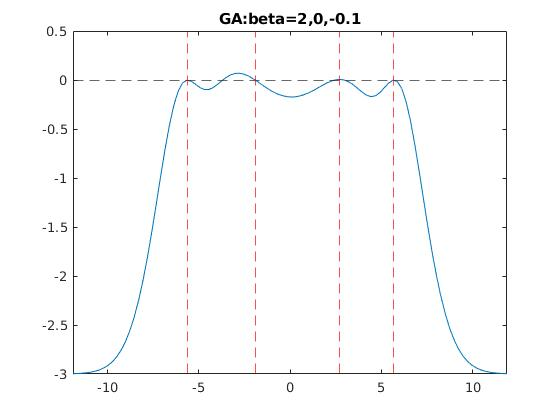
\includegraphics[scale=0.28]{quadplots/GA_1.jpg}
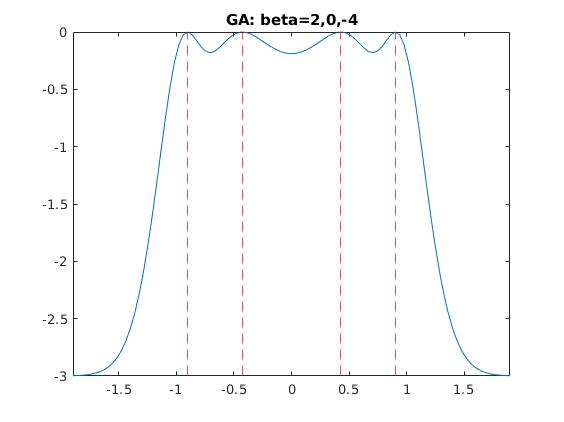
\includegraphics[scale=0.28]{quadplots/GA_2.jpg}\\
In the case when $\beta = (2,0,-0.1)^T$, the design produced by GA is not still not quite optimal. Parameter tuning?
\end{frame}


\begin{frame}{GA Results 2}
GA can also find the optimal 3 point designs.
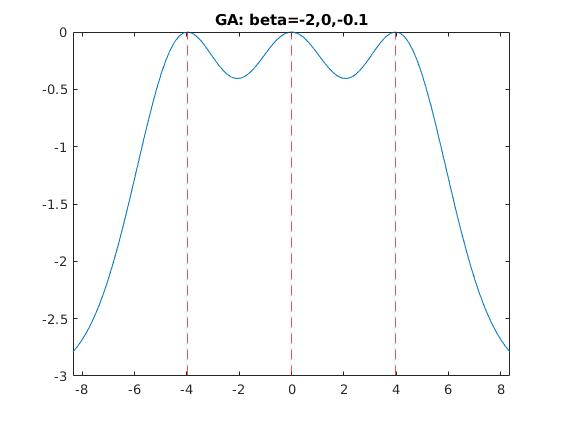
\includegraphics[scale=0.28]{quadplots/GA_3.jpg}
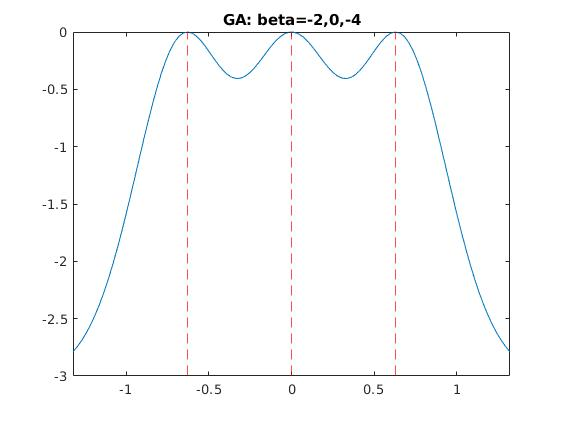
\includegraphics[scale=0.28]{quadplots/GA_4.jpg}
\end{frame}

\begin{frame}{Other Designs}
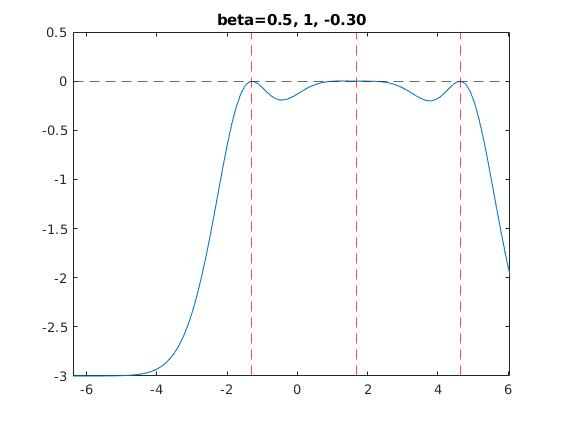
\includegraphics[scale=0.28]{quadplots/example_1.jpg}
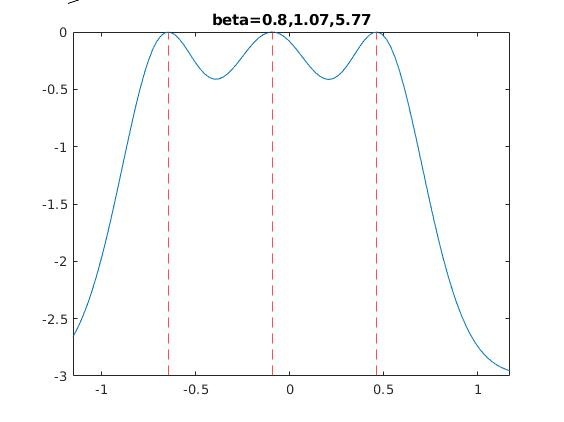
\includegraphics[scale=0.28]{quadplots/stackex.jpg}
\end{frame}

\begin{frame}{Optimal designs for quadratic model on any interval.}
The previous results were all for the case where $x \in (-\infty, \infty)$. What if the design interval was one of the following?
\begin{itemize}
\item $[0, \infty)$
\item $[-1, 1]$
\item $[a,b]$ where $a,b$ are larger than the optimal design points on $(-\infty, \infty)$.
\item $[0,1]$
\end{itemize}
I will use GA to find these optimal designs as GA seems to have better performance compared to PSO.
\end{frame}

\begin{frame}{$[0, \infty)$}
Strictly positive designs have 3 support points.\\
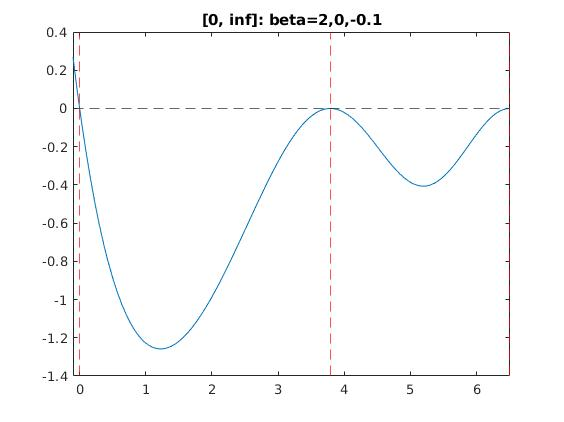
\includegraphics[scale=0.2]{quadplots/positive_1.jpg}
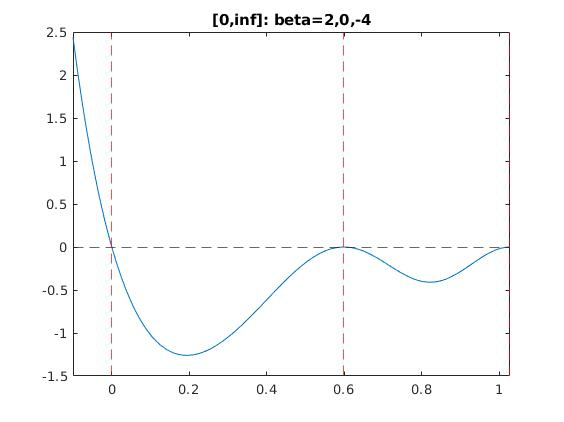
\includegraphics[scale=0.2]{quadplots/positive_2.jpg}\\
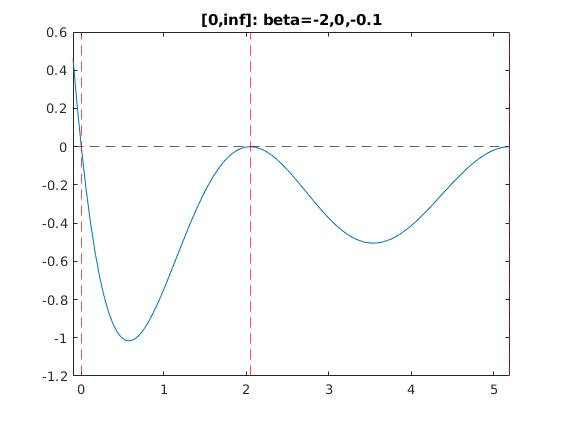
\includegraphics[scale=0.2]{quadplots/positive_3.jpg}
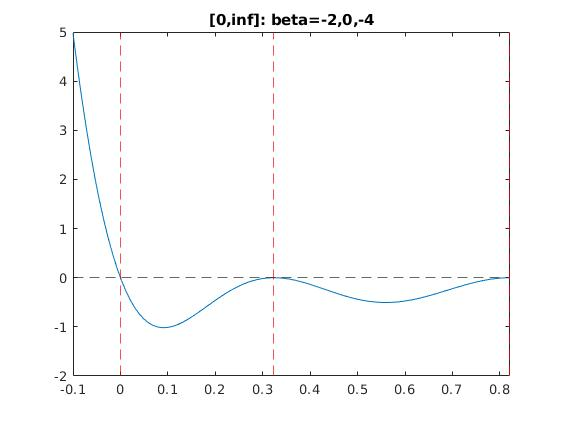
\includegraphics[scale=0.2]{quadplots/positive_4.jpg}
\end{frame}

\begin{frame}{$[-1, 1]$}
When beta = (2, 0,-4), the global optimal design points are already within the interval, so we get the 4 point design.\\
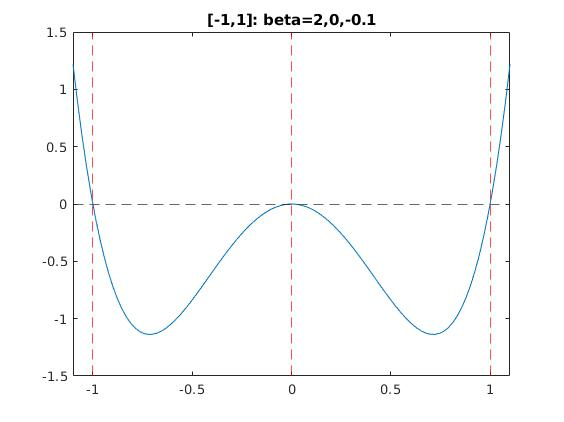
\includegraphics[scale=0.2]{quadplots/11_1.jpg}
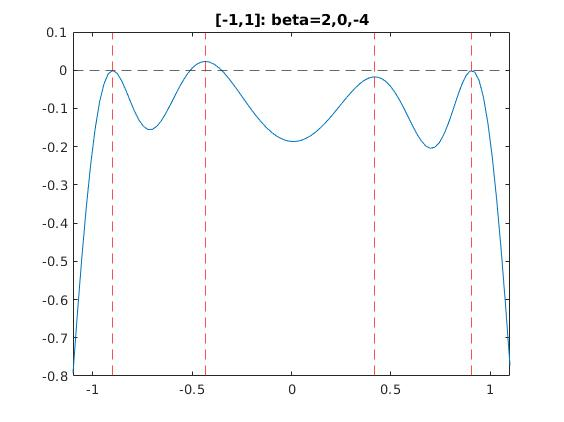
\includegraphics[scale=0.2]{quadplots/11_2.jpg}\\
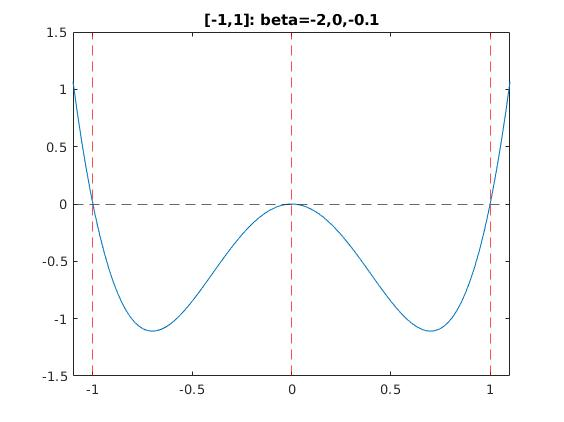
\includegraphics[scale=0.2]{quadplots/11_3.jpg}
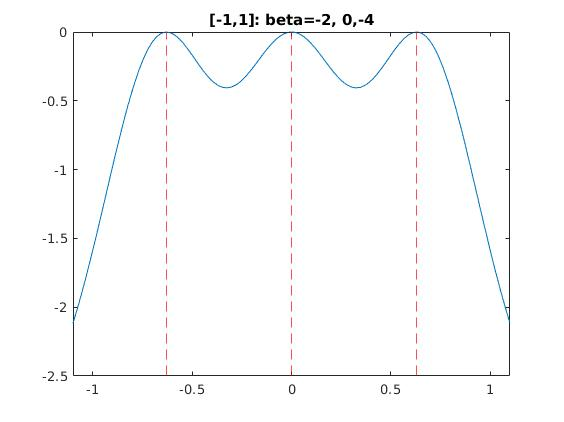
\includegraphics[scale=0.2]{quadplots/11_4.jpg}
\end{frame}

\begin{frame}{$[6,16]$}
beta=(2,0,-4) has issues. 1 point at 6 is close. Same with beta=(-2,0,-4). The two other nominal values are better.
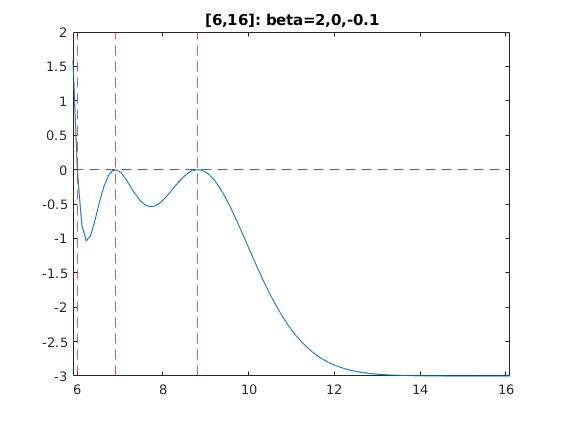
\includegraphics[scale=0.28]{quadplots/616_1.jpg}
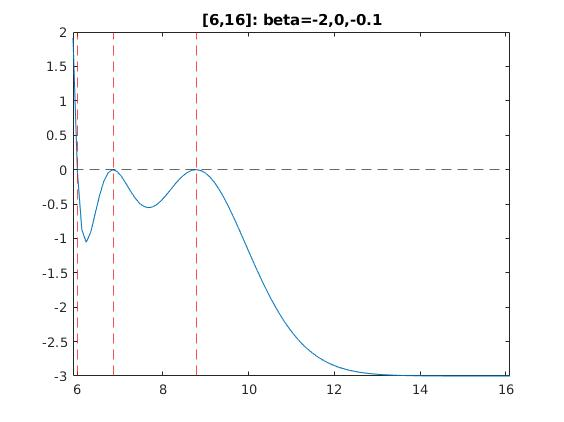
\includegraphics[scale=0.28]{quadplots/616_3.jpg}
\end{frame}

\begin{frame}{$[0,1]$}
Using the unit interval produces 3 point designs for out set of nominal values.\\
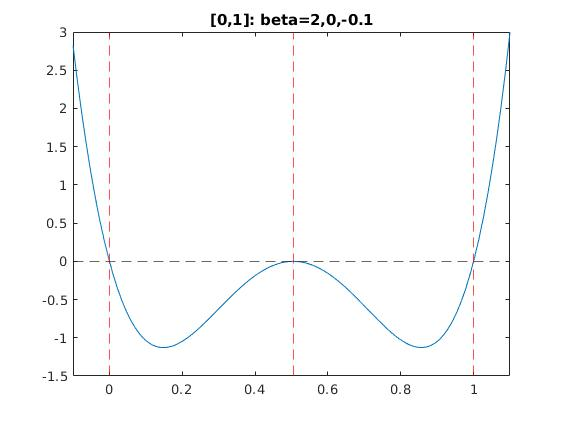
\includegraphics[scale=0.2]{quadplots/01_1.jpg}
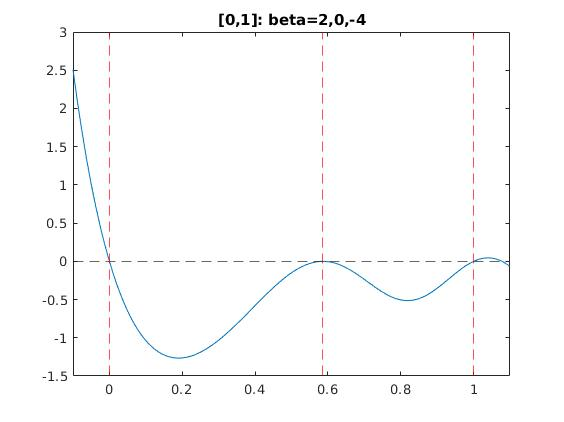
\includegraphics[scale=0.2]{quadplots/01_2.jpg}\\
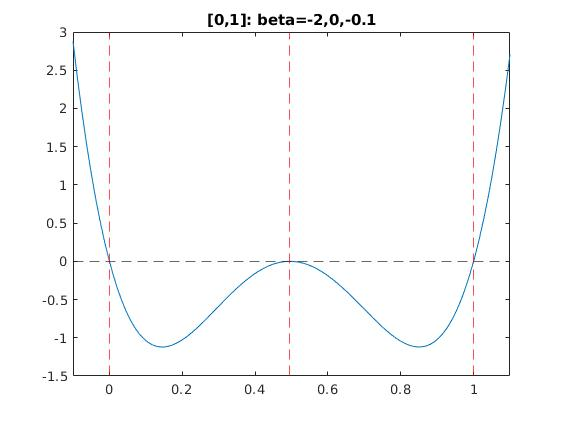
\includegraphics[scale=0.2]{quadplots/01_3.jpg}
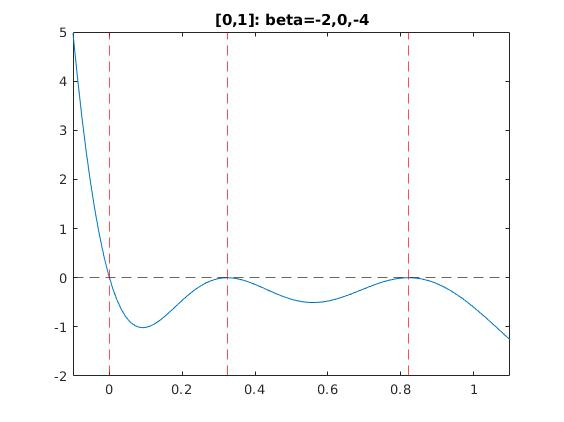
\includegraphics[scale=0.2]{quadplots/01_4.jpg}
\end{frame}

\begin{frame}{beta = (2, 0, -0.1)}
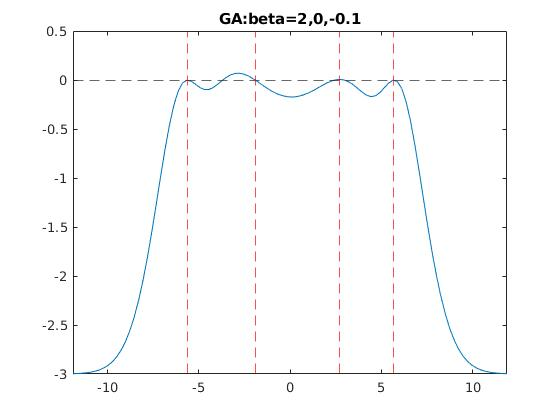
\includegraphics[scale=0.18]{quadplots/GA_1.jpg}
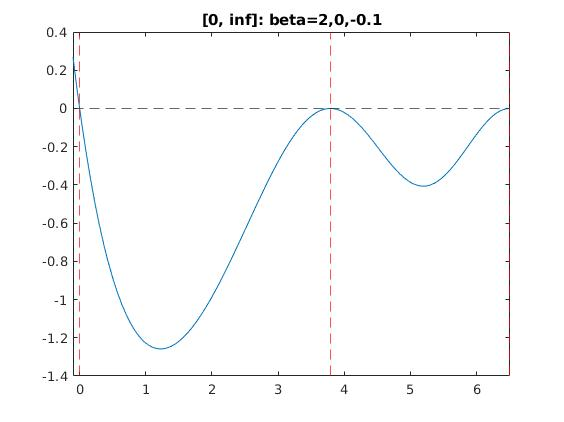
\includegraphics[scale=0.18]{quadplots/positive_1.jpg}
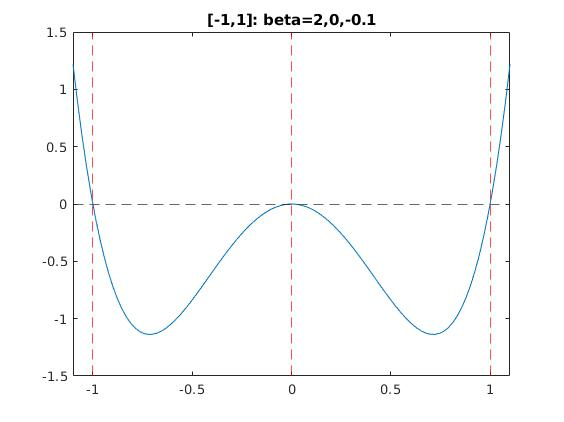
\includegraphics[scale=0.18]{quadplots/11_1.jpg}
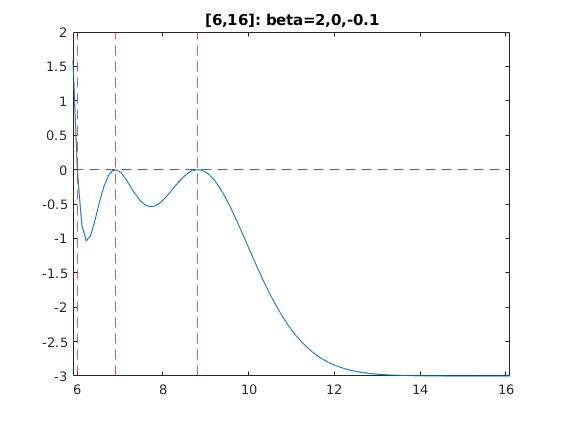
\includegraphics[scale=0.18]{quadplots/616_1.jpg}
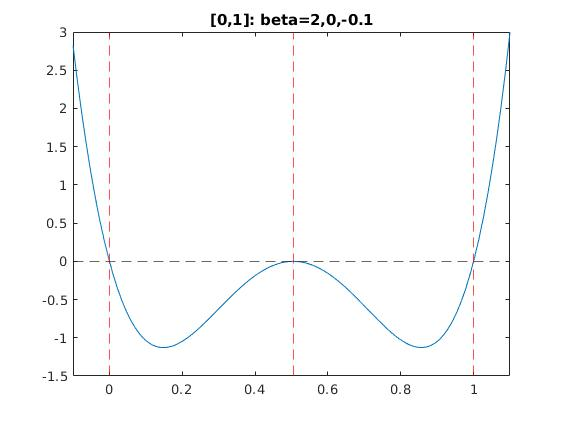
\includegraphics[scale=0.18]{quadplots/01_1.jpg}

\end{frame}

\begin{frame}{beta= (2,0,-4)}
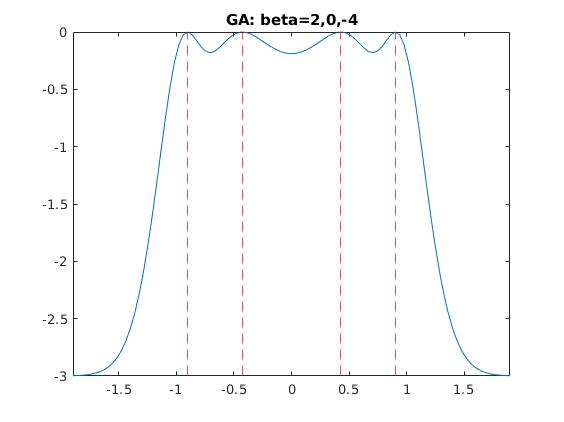
\includegraphics[scale=0.18]{quadplots/GA_2.jpg}
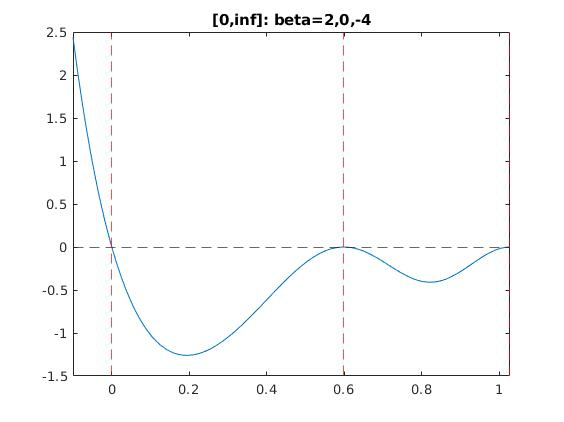
\includegraphics[scale=0.18]{quadplots/positive_2.jpg}
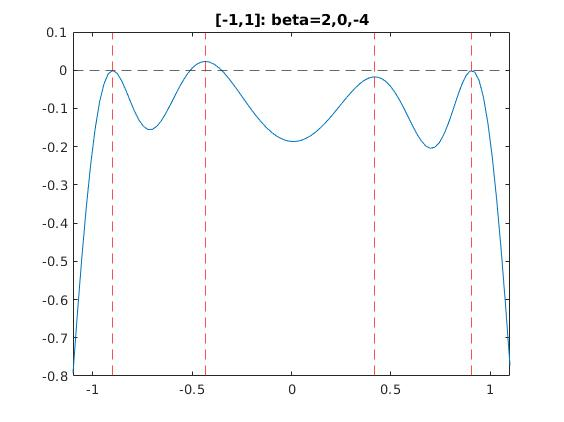
\includegraphics[scale=0.18]{quadplots/11_2.jpg}
%\includegraphics[scale=0.18]{quadplots/616_2.jpg}
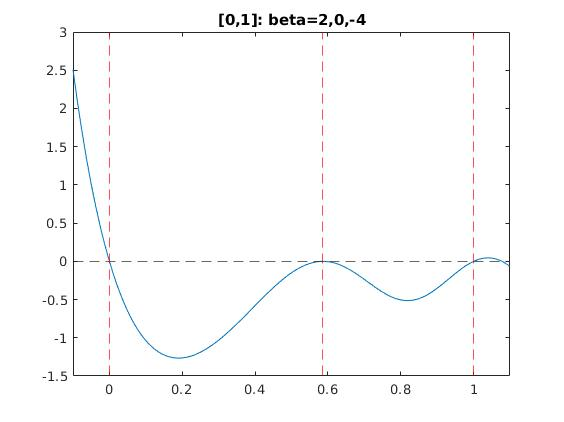
\includegraphics[scale=0.18]{quadplots/01_2.jpg}
\end{frame}

\begin{frame}{beta=(-2,0,-0.1)}
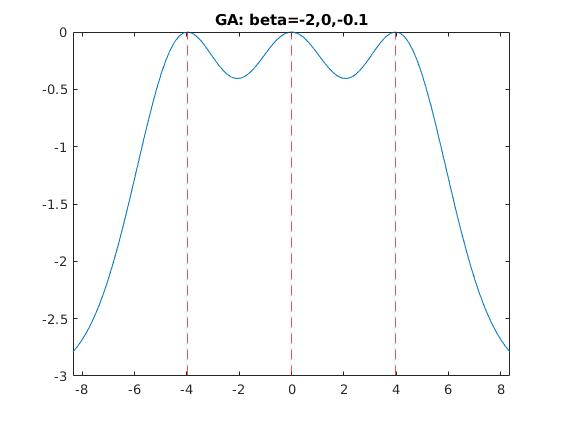
\includegraphics[scale=0.18]{quadplots/GA_3.jpg}
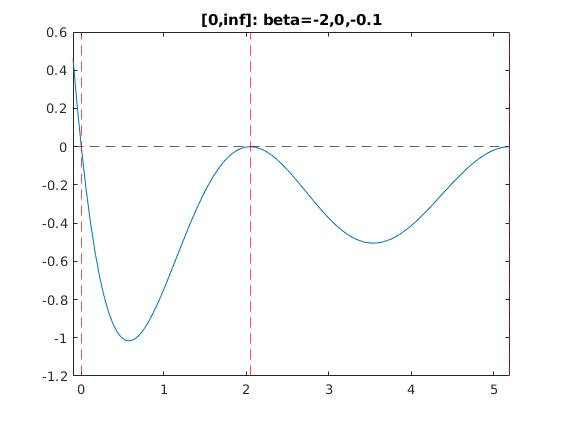
\includegraphics[scale=0.18]{quadplots/positive_3.jpg}
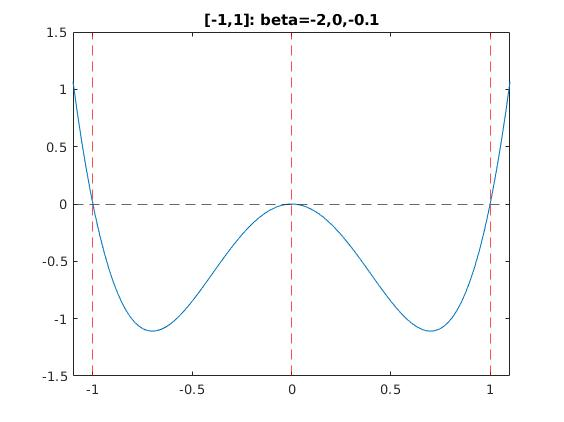
\includegraphics[scale=0.18]{quadplots/11_3.jpg}
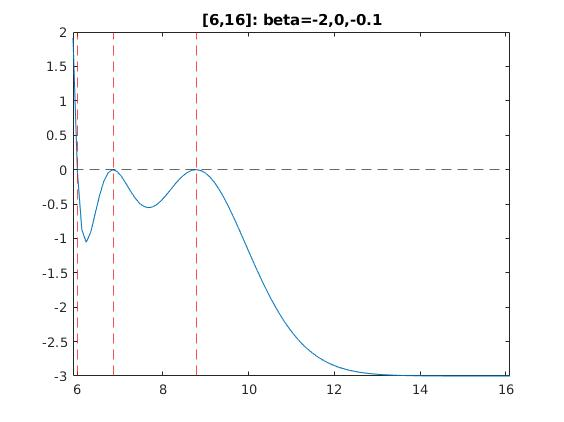
\includegraphics[scale=0.18]{quadplots/616_3.jpg}
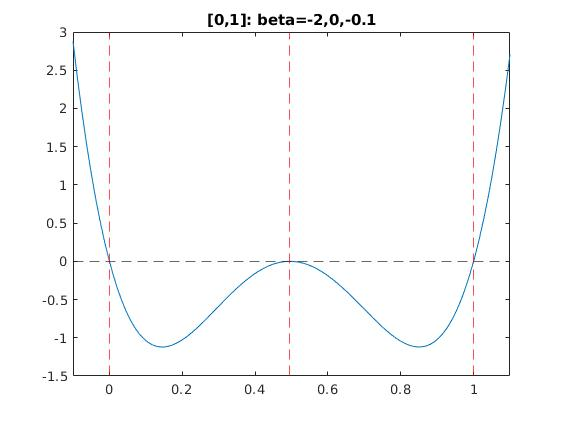
\includegraphics[scale=0.18]{quadplots/01_3.jpg}
\end{frame}

\begin{frame}{beta=(-2,0,-4)}
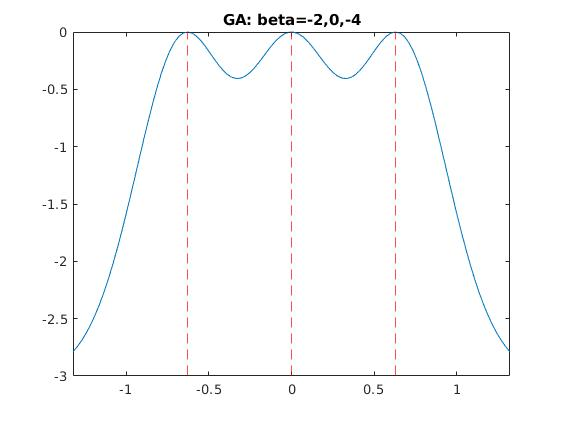
\includegraphics[scale=0.18]{quadplots/GA_4.jpg}
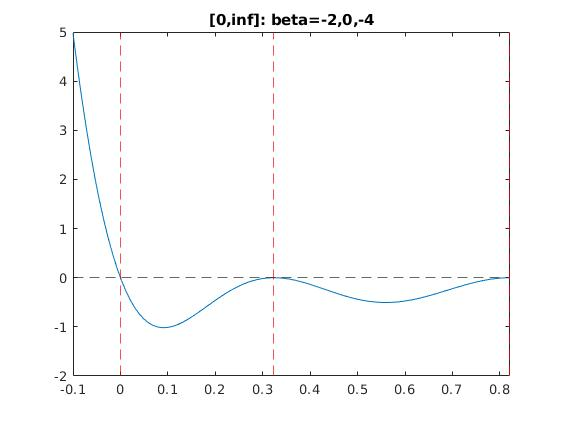
\includegraphics[scale=0.18]{quadplots/positive_4.jpg}
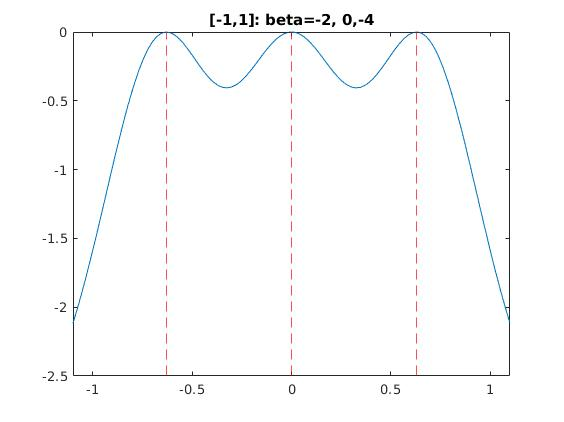
\includegraphics[scale=0.18]{quadplots/11_4.jpg}
%\includegraphics[scale=0.18]{quadplots/616_4.jpg}
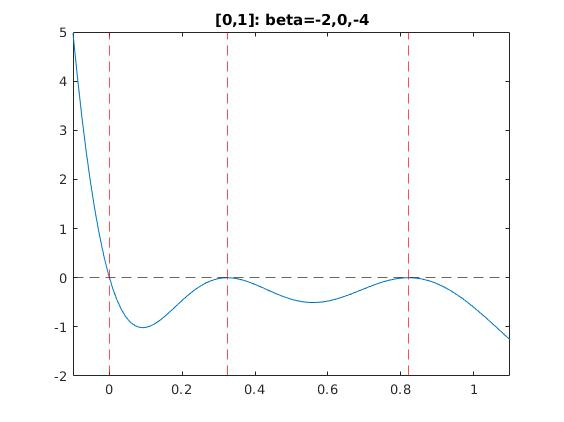
\includegraphics[scale=0.18]{quadplots/01_4.jpg}
\end{frame}

\begin{frame}{Conclusions}
\begin{itemize}
\item My code is able to replicate previous results for locally D-optimal designs.
\item Also is able to find designs on user-specified  design intervals.
\item Code can easily be extended to any degree polynomial.
\item Future work: fractional polynomials.
\item Demonstrate PlatEMO code.
\end{itemize}
\end{frame}

\begin{frame}{References}
\begin{itemize}
\item Paola Sebastiani, Raffaella Settimi (1997),
\textit{A note on D-optimal designs for a logistic regression model},
Journal of Statistical Planning and Inference
\item Shwetank Lall, Seema Jaggi, Eldho Varghese, Cini Varghese \& Arpan
Bhowmik (2018): \textit{An algorithmic approach to construct D-optimal saturated designs for logistic
model}, Journal of Statistical Computation and Simulation
\item Thomas Mathew, Bikas Kumar Sinha (2001),
\textit{Optimal designs for binary data under logistic regression},
Journal of Statistical Planning and Inference
\item Ellinor Fornius (2005), \textit{D-optimal Designs for Quadratic Logistic Regression Models}
\end{itemize}
\end{frame}
%\begin{frame}{Results from Mathew, Sinha}
%Mathew, Sinha (2001) derive several optimal designs for the 2 parameter logistic model.
%\begin{itemize}
%\item D-optimal: equal weights at $\frac{\pm 1.5434 - \beta_0}{\beta_1}$
%\item A-optimal: found best 2 point design.
%\end{itemize}
%Not addressed: A-optimal design within class of all designs and E-optimal designs. Also, no sensitivity plots to confirm optimality graphically.
%
%\end{frame}
%
%\begin{frame}{Results from Lall et al.}
%Lall et. al (2018) uses a modified Fedorov algorithm to construct saturated D-optimal designs for several 1 and 2 variable logistic models on the design interval $[-1,1]$. The following table shows their designs for the 1 variable model.
%\begin{center}
%\begin{tabular}{|c|c|c|c|}
%\hline 
% $\beta_0$ & $\beta_1$ & $x_1$ & $x_2$ \\ 
%\hline 
% 0.1 & 0.5 & -1 & 1 \\ 
%\hline 
% 1 & 1 & -1 & 1 \\ 
%\hline 
% 1 & 4 & -0.636 & 0.136 \\ 
%\hline 
%\end{tabular} 
%\end{center}
%Since these are saturated designs, both support points have equal weights.
%
%Their algorithm relies on a discretized design space, which makes it difficult to apply to global optimality.
%
%\end{frame}
%
%\begin{frame}{Results from Sebastiani}
%Sebastiani (1992) derives D-optimal designs for the 1 variable model for an unbounded, bounded design interval, and for a design interval bounded at a single end.
%\begin{itemize}
%\item Designs for bounded intervals are modified versions of the global optimum.
%\item If the ideal design point is outside of the bound, the bound will be one of the design points.
%\end{itemize}
%
%Results for $\beta_0 = 0$, $\beta_1 = 1$:
%\begin{center}
%\begin{tabular}{|c|c|c|c|c|c|}
%\hline 
%  & $[-\infty, \infty]$  & $[-1, \infty]$ & $[-\infty,1]$ & $[-1,1]$ & $[10, 20]$\\ 
%\hline 
%$x_1$ & -1.543 & -1 & -1.796 & -1  & 10.00\\ 
%\hline 
%$x_2$ & 1.543 & 1.796 & 1 & 1 & 12.00\\ 
%\hline 
%\end{tabular} 
%\end{center}
%All designs are equally weighted.
%
%\end{frame}
%
%\begin{frame}{Results from Fornius}
%Fornious (2005) derives D-optimal designs for the quadratic model with $\eta_i = \beta_0 + \beta_1 x_i + \beta_2 x_i^2$. Designs have either 3 or 4 support points depending on shape of response.
%
%\begin{tabular}{|c|c|}
%\hline 
% Nominal values & Design \\ 
%\hline 
% $2,0,-0.1$ & 
%$\begin{bmatrix}
%-5.7185 & -2.7017  & 2.7017 & 5.7185\\
%0.3138 & 0.1862 & 0.1862 & 0.3138
%\end{bmatrix}$  \\ 
%\hline 
% $2,0,-4$ & $\begin{bmatrix}
%-0.9042 & -0.4272  & 0.4272 & 0.9042\\
%0.3138 & 0.1862 & 0.1862 & 0.3138
%\end{bmatrix}$   \\ 
%\hline 
% $-2,0,-0.1$ & 
%$\begin{bmatrix}
%-3.9819 & 0  & 3.9819\\
%1/3 & 1/3 & 1/3
%\end{bmatrix}$   \\ 
%\hline 
% $-2,0,-4$ & 
%$\begin{bmatrix}
%-0.6296 & 0  & 0.6296\\
%1/3 & 1/3 & 1/3
%\end{bmatrix}$  \\ 
%\hline 
%\end{tabular} \\
%What happens when $\beta_1 \neq 0$? $\implies$ just shifts solution What about on different design intervals?
%\end{frame}



\end{document}